% Slides for talk on hydrogen fuel cells
% given in the department on October 27, 2003.
% 
% The original slides were in Prosper.  This file contains the
% translation of the original slides to Beamer.
% 
% Rouben Rostamian <rostamian@umbc.edu>
% August 31, 2004

\documentclass[10pt]{beamer}
\usetheme{umbc4}

\useinnertheme{umbcboxes}
\setbeamercolor{umbcboxes}{bg=violet!12,fg=black}

\usepackage{rotating} % for defining \schwa
\newcommand{\schwa}{\raisebox{1ex}{\begin{turn}{180}e\end{turn}}}

\newcommand{\arcsinh}{\mathop\mathrm{arcsinh}\nolimits}
\newcommand{\arccosh}{\mathop\mathrm{arccosh}\nolimits}
\newcommand{\Pu}{P_{\mathrm{amb}}}

\title{Openyoudao}
% \subtitle{Modeling and Computations}
% \author[R. Rostamian]{Rouben Rostamian}
\title{A story about Openyoudao}
\date{September 17, 2012}
\begin{document}

%----------- titlepage ----------------------------------------------%
\begin{frame}[plain]
  \titlepage
\end{frame}

%----------- slide 
%--------------------------------------------------%
\begin{frame}
  \frametitle{I am a freshman}

\begin{center} 
  
\includegraphics[width=0.8\textwidth]{newer.jpg}
\end{center}
\medskip
\quad
\qquad

I am linuxer, Reading paper just so boring, I can't bear it any more!!!
\end{frame}

%----------- slide
%--------------------------------------------------%
\begin{frame}
  \frametitle{History 2012--04--16 A boring Day!!!}

\begin{center} 
  
\includegraphics[width=0.4\textwidth]{pic1.jpg}
\end{center}
\medskip
\quad
\qquad

I am linuxer, Reading paper just so boring, I can't bear it any more!!!
\end{frame}

%----------- slide --------------------------------------------------%
\begin{frame}
  \frametitle{Why reading paper on linux just so diffcult?}

\begin{center} 
  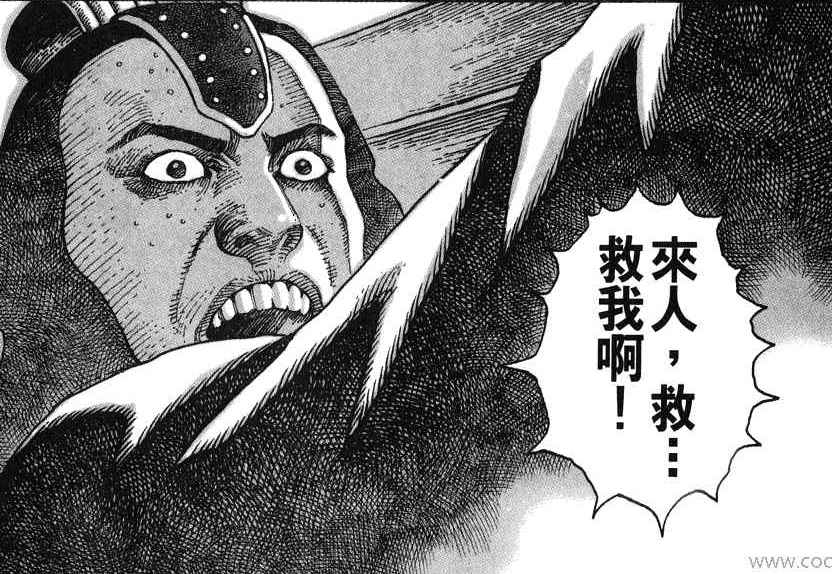
\includegraphics[width=0.6\textwidth]{help.jpg}
\end{center}

\end{frame}

%----------- slide --------------------------------------------------%
\begin{frame}
  \frametitle{Fuck! Writing a dictionary by myself}
 
\begin{center} 
  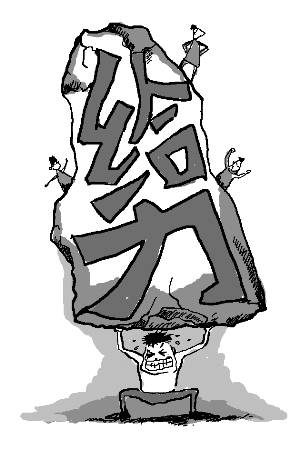
\includegraphics[width=0.4\textwidth]{geili.jpg}
  
\end{center}

\end{frame}

%----------- slide --------------------------------------------------%
\begin{frame}
  \frametitle{2012--05--28 A new life born: Openyoudao v0.1}

\begin{center} 
  
\includegraphics[width=0.6\textwidth]{newlife.jpg}
\href{run:youdao-v0.1.mp4}{\beamerbutton{Openyoudao v0.1}}

\end{center}

\end{frame}

%----------- slide --------------------------------------------------%
\begin{frame}
  \frametitle{the structure  of openyoudao}
\begin{center} 
  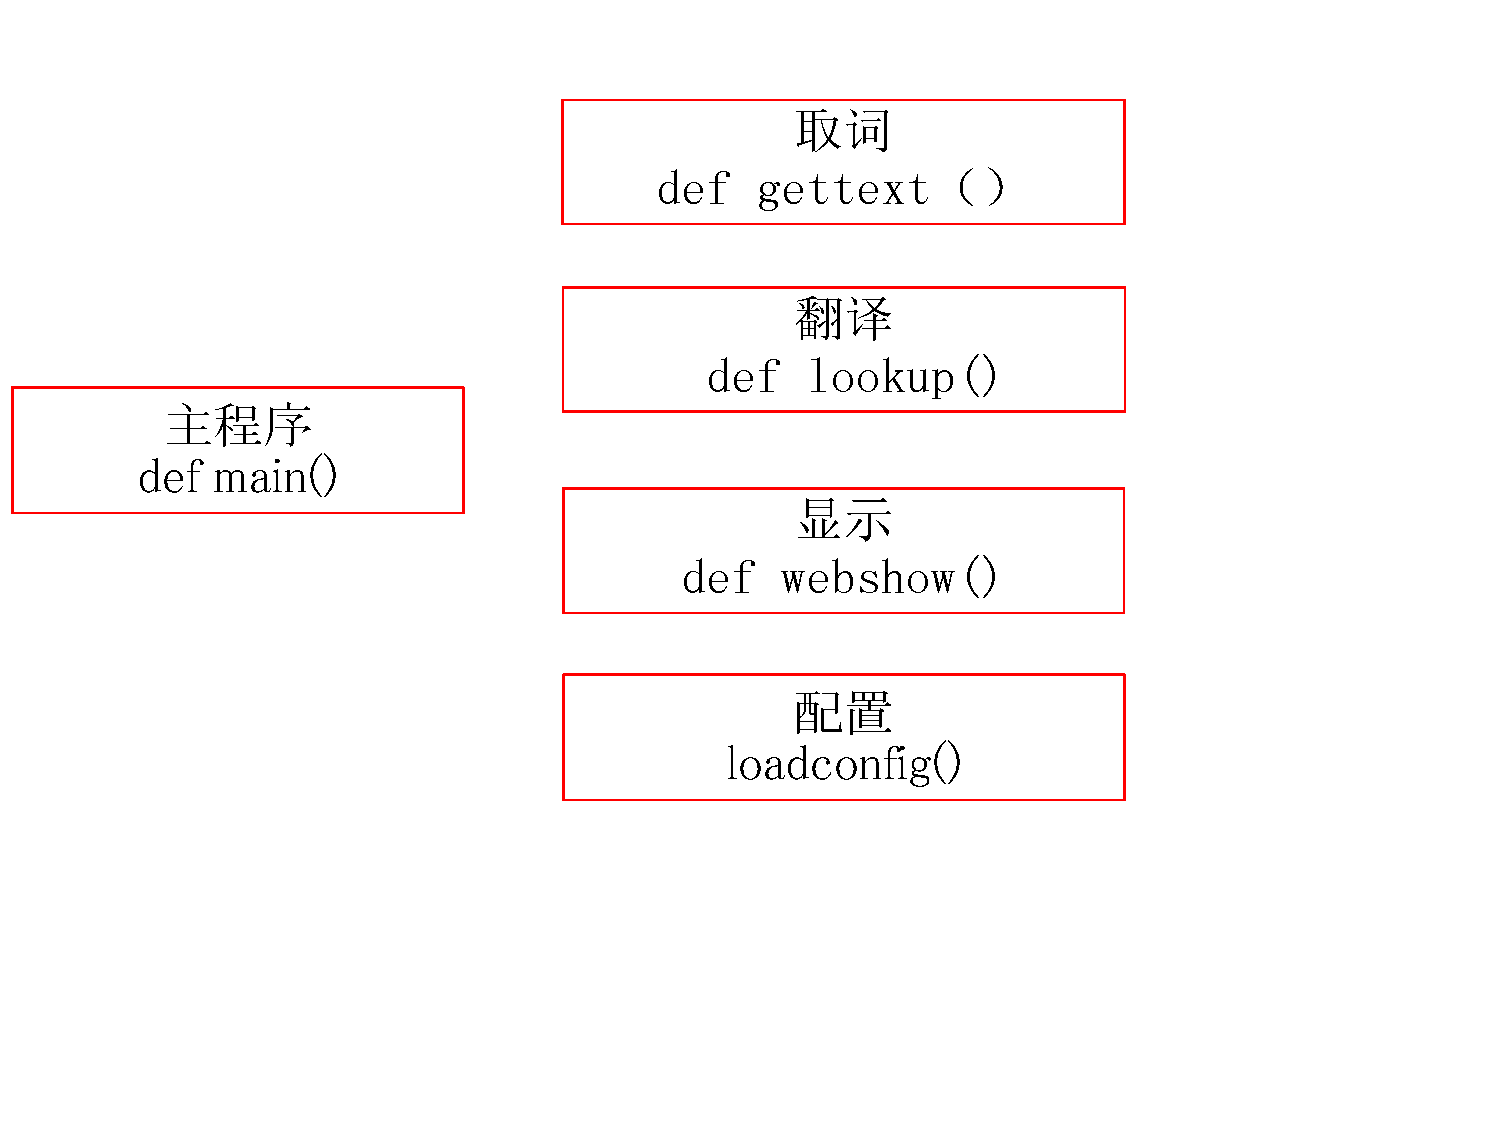
\includegraphics[width=1.1\textwidth]{construct.pdf}

\end{center}

\end{frame}

%----------- slide --------------------------------------------------%
\begin{frame}
  \frametitle{What shold i do? if i want to complete this program?}
\begin{center} 
  
\includegraphics[width=1.\textwidth]{myfirststep.jpg}

\end{center}

\end{frame}
%----------- slide --------------------------------------------------%
\begin{frame}
  \frametitle{The question ask to my self}
\begin{itemize}
  \item What should i do first?
  \item How to take the word that i want?
  \item How to translate it?
  \item How to show it?
\end{itemize}
\end{frame}

%----------- slide --------------------------------------------------%
\begin{frame}
  \frametitle{The fun of programming}
  
\begin{center} 
  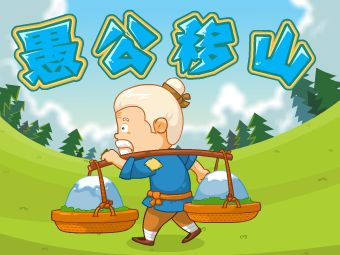
\includegraphics[width=0.7\textwidth]{challenge.jpg}

\end{center}

\end{frame}

%----------- slide  --------------------------------------------------%
\begin{frame}
  \frametitle{what I have learn in this process?}
\begin{itemize}
  \item python 
  \item git
  \item bash
  \item js/jquery
  \item sqlite
  \item pip
  \item file lock
  \item soft break
\end{itemize}

\end{frame}

%----------- slide --------------------------------------------------%
\begin{frame}
  \frametitle{To do Next... }
\textbf Give me your suggestion...

\end{frame}

%----------- slide --------------------------------------------------%
\begin{frame}
  \frametitle{what is opensource?}


\end{frame}

%----------- slide --------------------------------------------------%
\begin{frame}
  \frametitle{How to Join Us?}

http://openyoudao.org/\\
https://github.com/justzx2011/openyoudao\\
justzx2011@gmail.com  @justzx\\
lvzongting@gmail.com  @lvzongting\\

\end{frame}

%----------- slide --------------------------------------------------%
\begin{frame}
  \frametitle{Thanks}
\begin{center} 
  
\includegraphics[width=0.6\textwidth]{thanks.png}
\end{center}
\end{frame}

%----------- slide 
\end{document}
